% main.tex - viza701 paper, group 5. overleaf, pdflatex + bibtex
% sections in sections/, figs in figures/ (make figures fills it from the repo)
\documentclass[11pt,letterpaper]{article}
\usepackage[margin=1in]{geometry}
\usepackage[utf8]{inputenc}
\usepackage[T1]{fontenc}
\usepackage{graphicx}
\usepackage{amsmath}
\usepackage{booktabs}
\usepackage{natbib}
\usepackage{hyperref}
\usepackage{xcolor}
\usepackage{caption}
\captionsetup{font=small,labelfont=bf}
\graphicspath{{figures/}}
\hypersetup{colorlinks=true,linkcolor=black,citecolor=blue!60!black,urlcolor=blue!60!black}

% header stuff, TODO put the real UINs
\newcommand{\myname}{Omar Khattab and Arash Baghipour Aliabadi}
\newcommand{\myuin}{UIN: 000000000 (Omar), 000000000 (Arash)}
\newcommand{\mycourse}{VIZA 701: Introduction to Research in Visual Computing and Interactive Media}
\newcommand{\myinstructor}{Instructor: Dr. Suryansh Kumar}

\title{How much science survives the shot?\\
\large Measuring cinematic rendering choices against astronomical data cubes}
\author{\myname\\[2pt] \small \myuin\\ \small \mycourse\\ \small \myinstructor}
\date{December 4, 2026}

\begin{document}
\maketitle

\begin{abstract}
% abstract, me, write it last. 1 paragraph: zero point, 16 operators scored on real cube + fake disk, depth index, safe envelope
TODO abstract. zero point (plain render == moment0), 16 operators on l1448 + disk, 1 sentence per result (ranking, band crossings, orbit cost, index + envelope).

\end{abstract}

\section{Introduction}
% arash. the oct 30 motivation but as text: even pillars of creation is 3 filters painted into colors,
% people cant tell which parts are data (jensen 2024: 90 / 68 / 26 %), color flips what they
% conclude (smith 2011: 71.5 %), 3 pipeline stages get checked and the render doesnt.
% end with the research question + the 3 contributions
\label{sec:intro}

\begin{figure}[t]
  \centering
  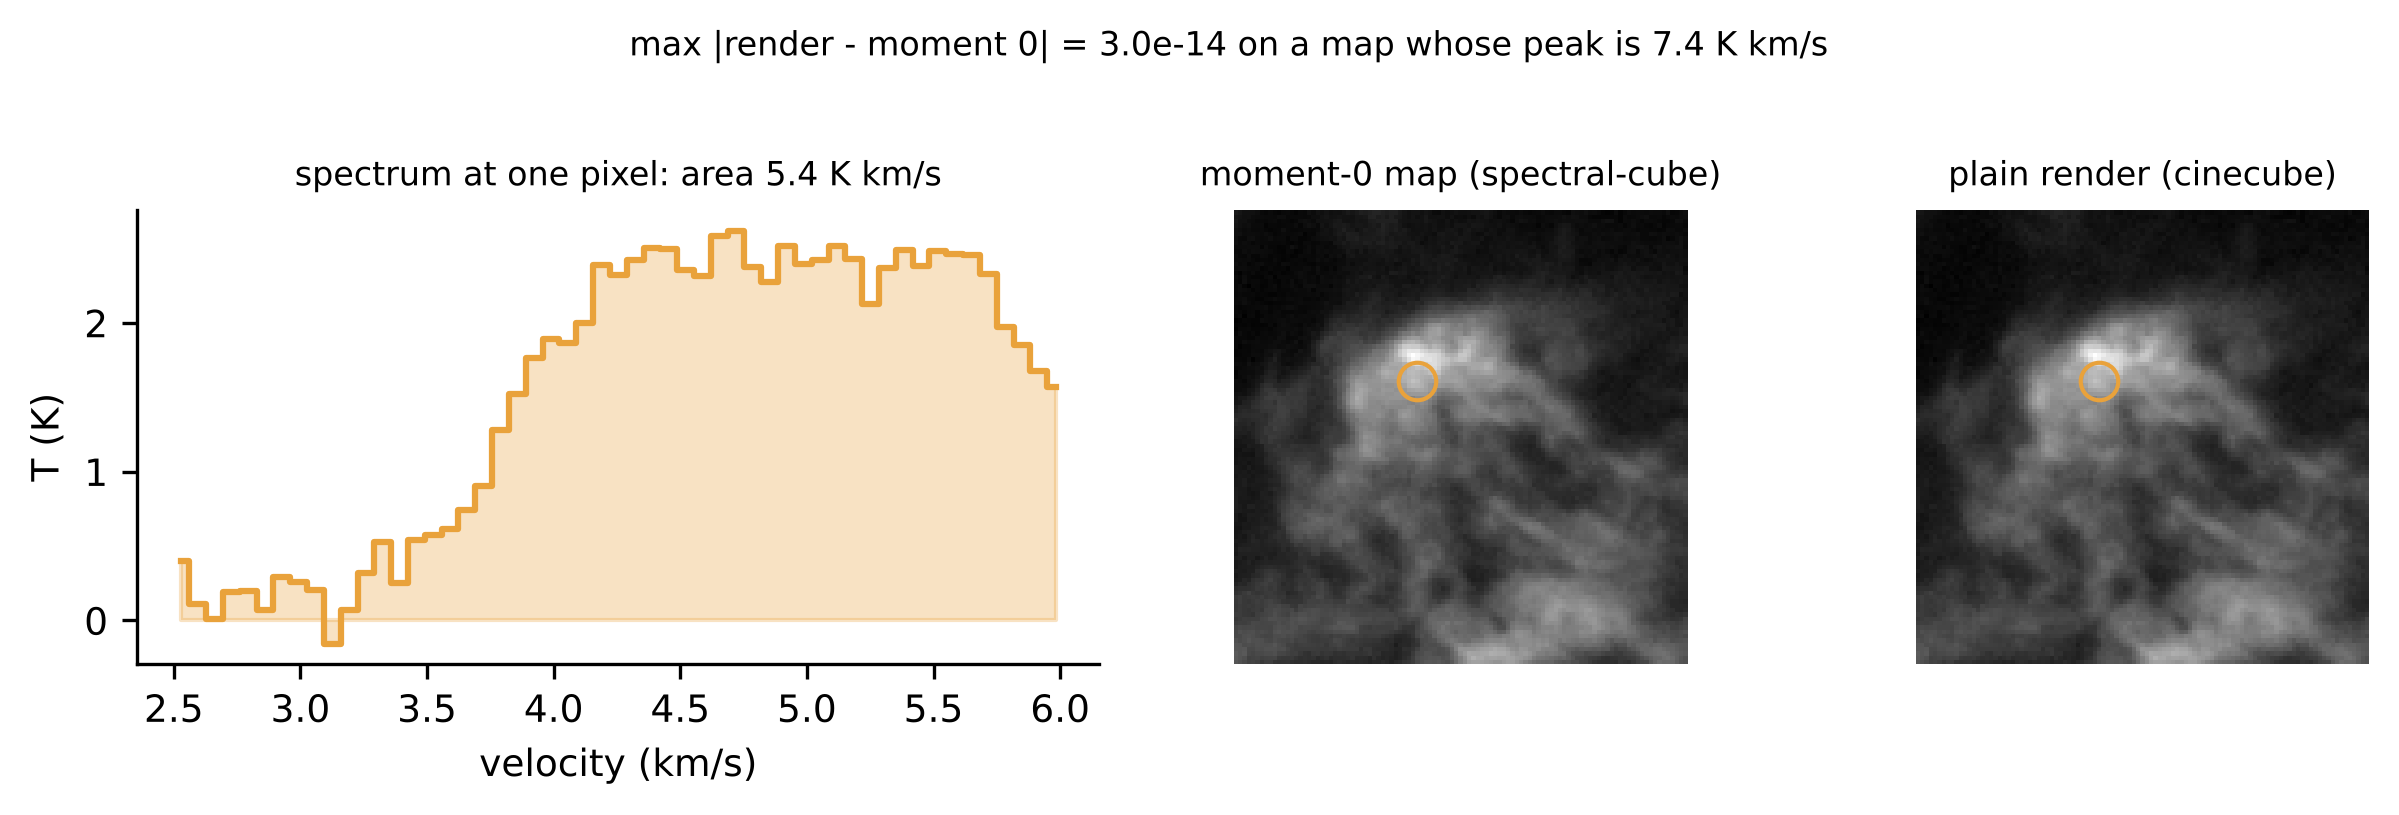
\includegraphics[width=\linewidth]{fig_equivalence}
  % TODO real caption. left: spectrum at 1 pixel + area under it, mid: moment0 from spectral-cube, right: our plain render. diff 3e-14 on a map peaking at 7.4 K km/s
  \caption{The zero point: moment-0 map (middle) vs the plain render (right), spectrum at one pixel on the left.}
  \label{fig:equivalence}
\end{figure}

\section{Related work}
% arash. 4 threads, 1 paragraph each, only cite stuff we actually opened:
% cinematic sci vis + audiences (borkiewicz 2019, jensen 2024, stepanovic 2024)
% cube tools + the caveats they say themselves (taylor 2025, sivitilli 2026, litaker 2013)
% fidelity / reconstruction metrics (kindlmann 2014, bujack 2026, max 1995, peters 2014)
% velocity space projection effects (beaumont 2013)
\label{sec:related}

\section{Method}
% arash + me. basically docs/metrics.md from the repo. subsections below, max 2 pages
\label{sec:method}

\subsection{Data}
% l1448 (fcrao complete, ridge 2006) + the fake keplerian disk (cinecube.synth)

\subsection{The reference render and the equivalence}
% emission only render integral. linear TF, no absorption, ortho camera down the v axis
% -> sum_v T dv = moment0. same eq with physical coefficients = radiative transfer w/o
% scattering (max 1995, peters 2014)
\begin{equation}
  I(x,y) \;=\; \sum_{v} T(x,y,v)\,\Delta v \;=\; M_0(x,y)
  \label{eq:equivalence}
\end{equation}

\subsection{Cinematic operators}
% 8 families, each a pure function with logged params, expected failure class per family

\subsection{Decoding a frame back to data}
% quantize, display noise, nearest colormap color in CIELAB (bujack 2026), blind vs informed

\subsection{Scores, controls and bands}
% data recovered (spearman over sky mask), structure kept (ssim), flux visible, the 5 controls, bands

\subsection{The synthetic disk and the velocity-as-depth index}
% disk model, 2 worlds same camera, index = 1 - ssim between ppv render and true density render

\section{Results}
% me. 1 finding per paragraph with its number, everything from results/frozen/
\label{sec:results}

\begin{figure}[t]
  \centering
  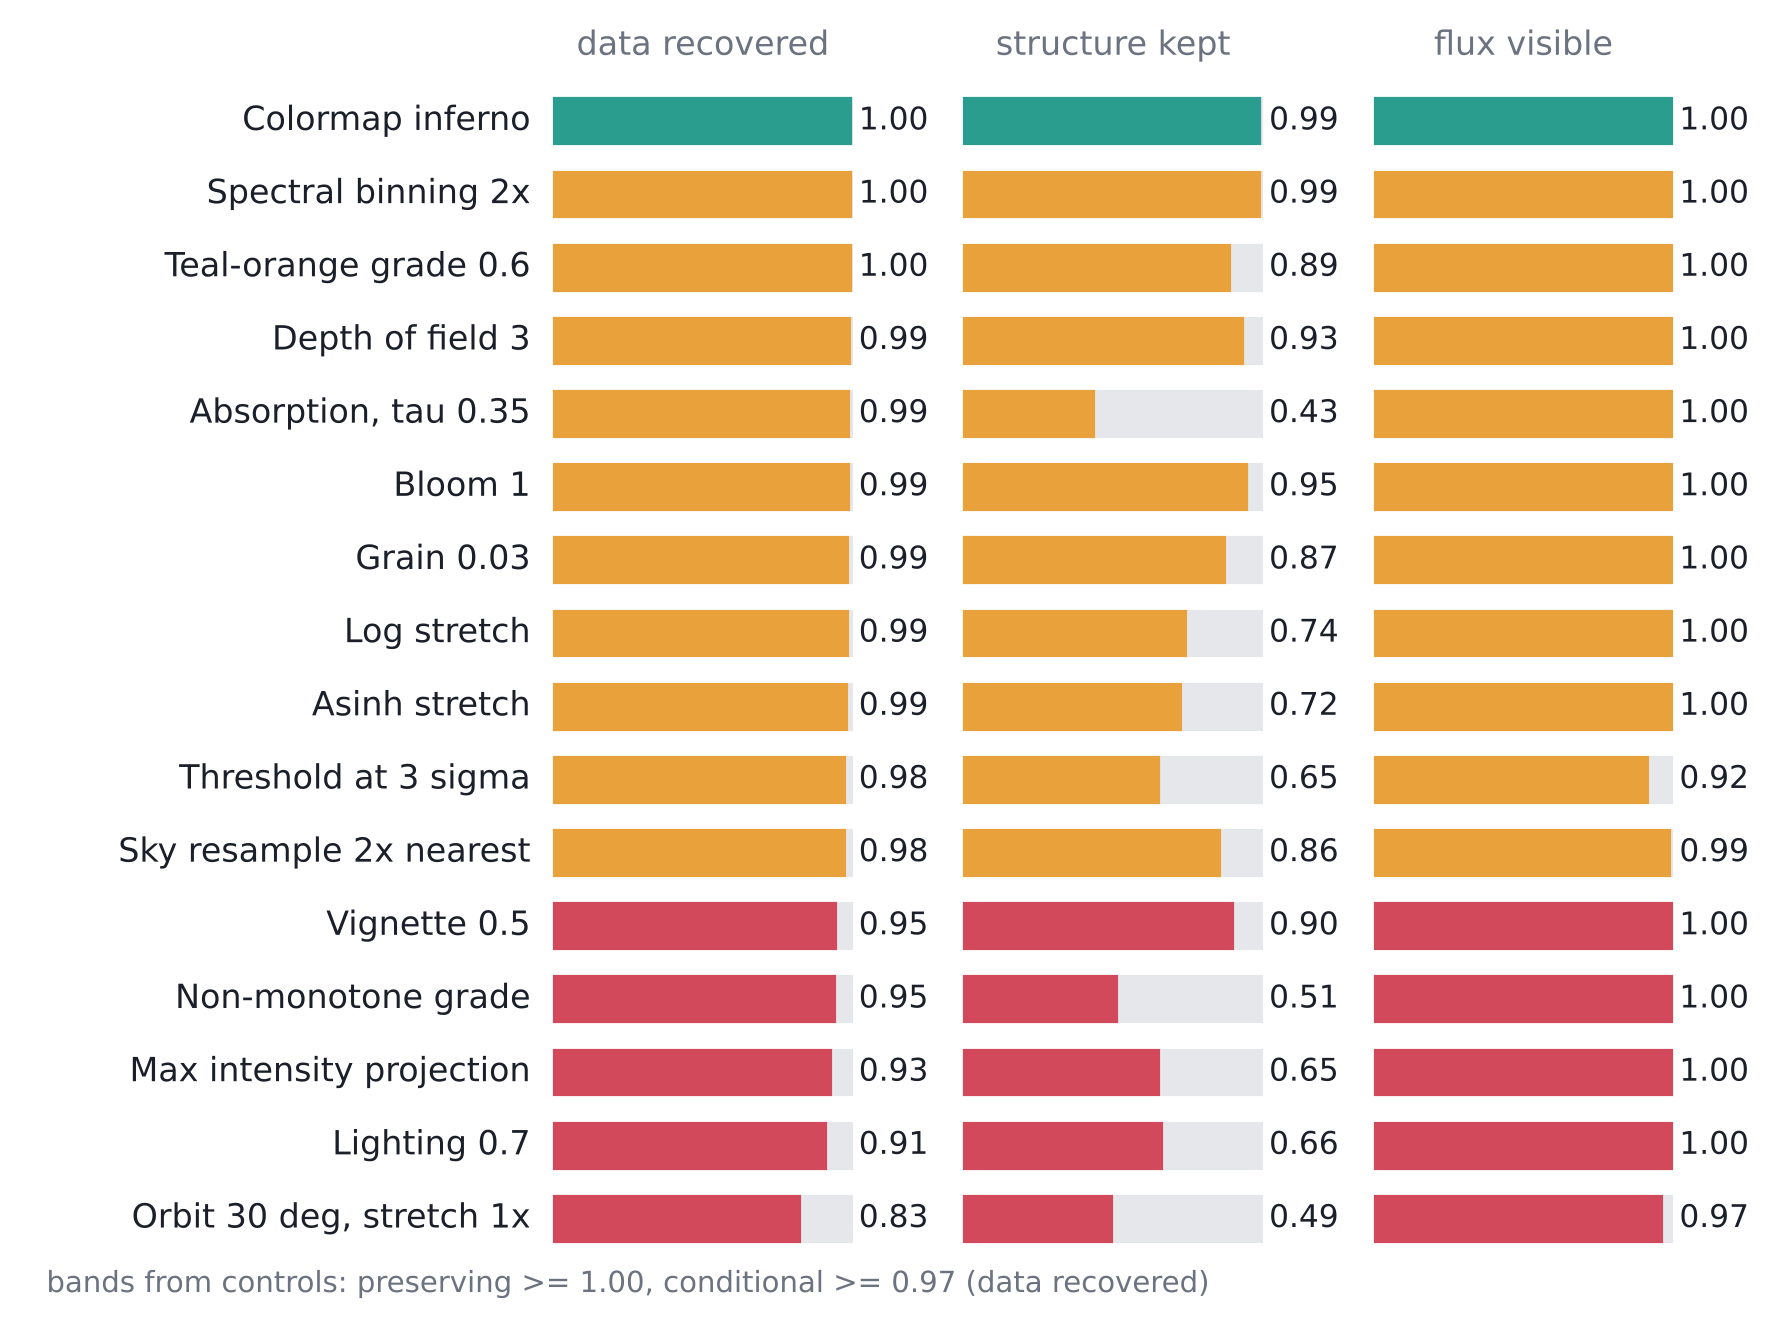
\includegraphics[width=\linewidth]{fig_ladder_l1448}
  % TODO caption
  \caption{Operators ranked by data recovered on L1448 (bars colored by band).}
  \label{fig:ladder}
\end{figure}

\begin{figure}[t]
  \centering
  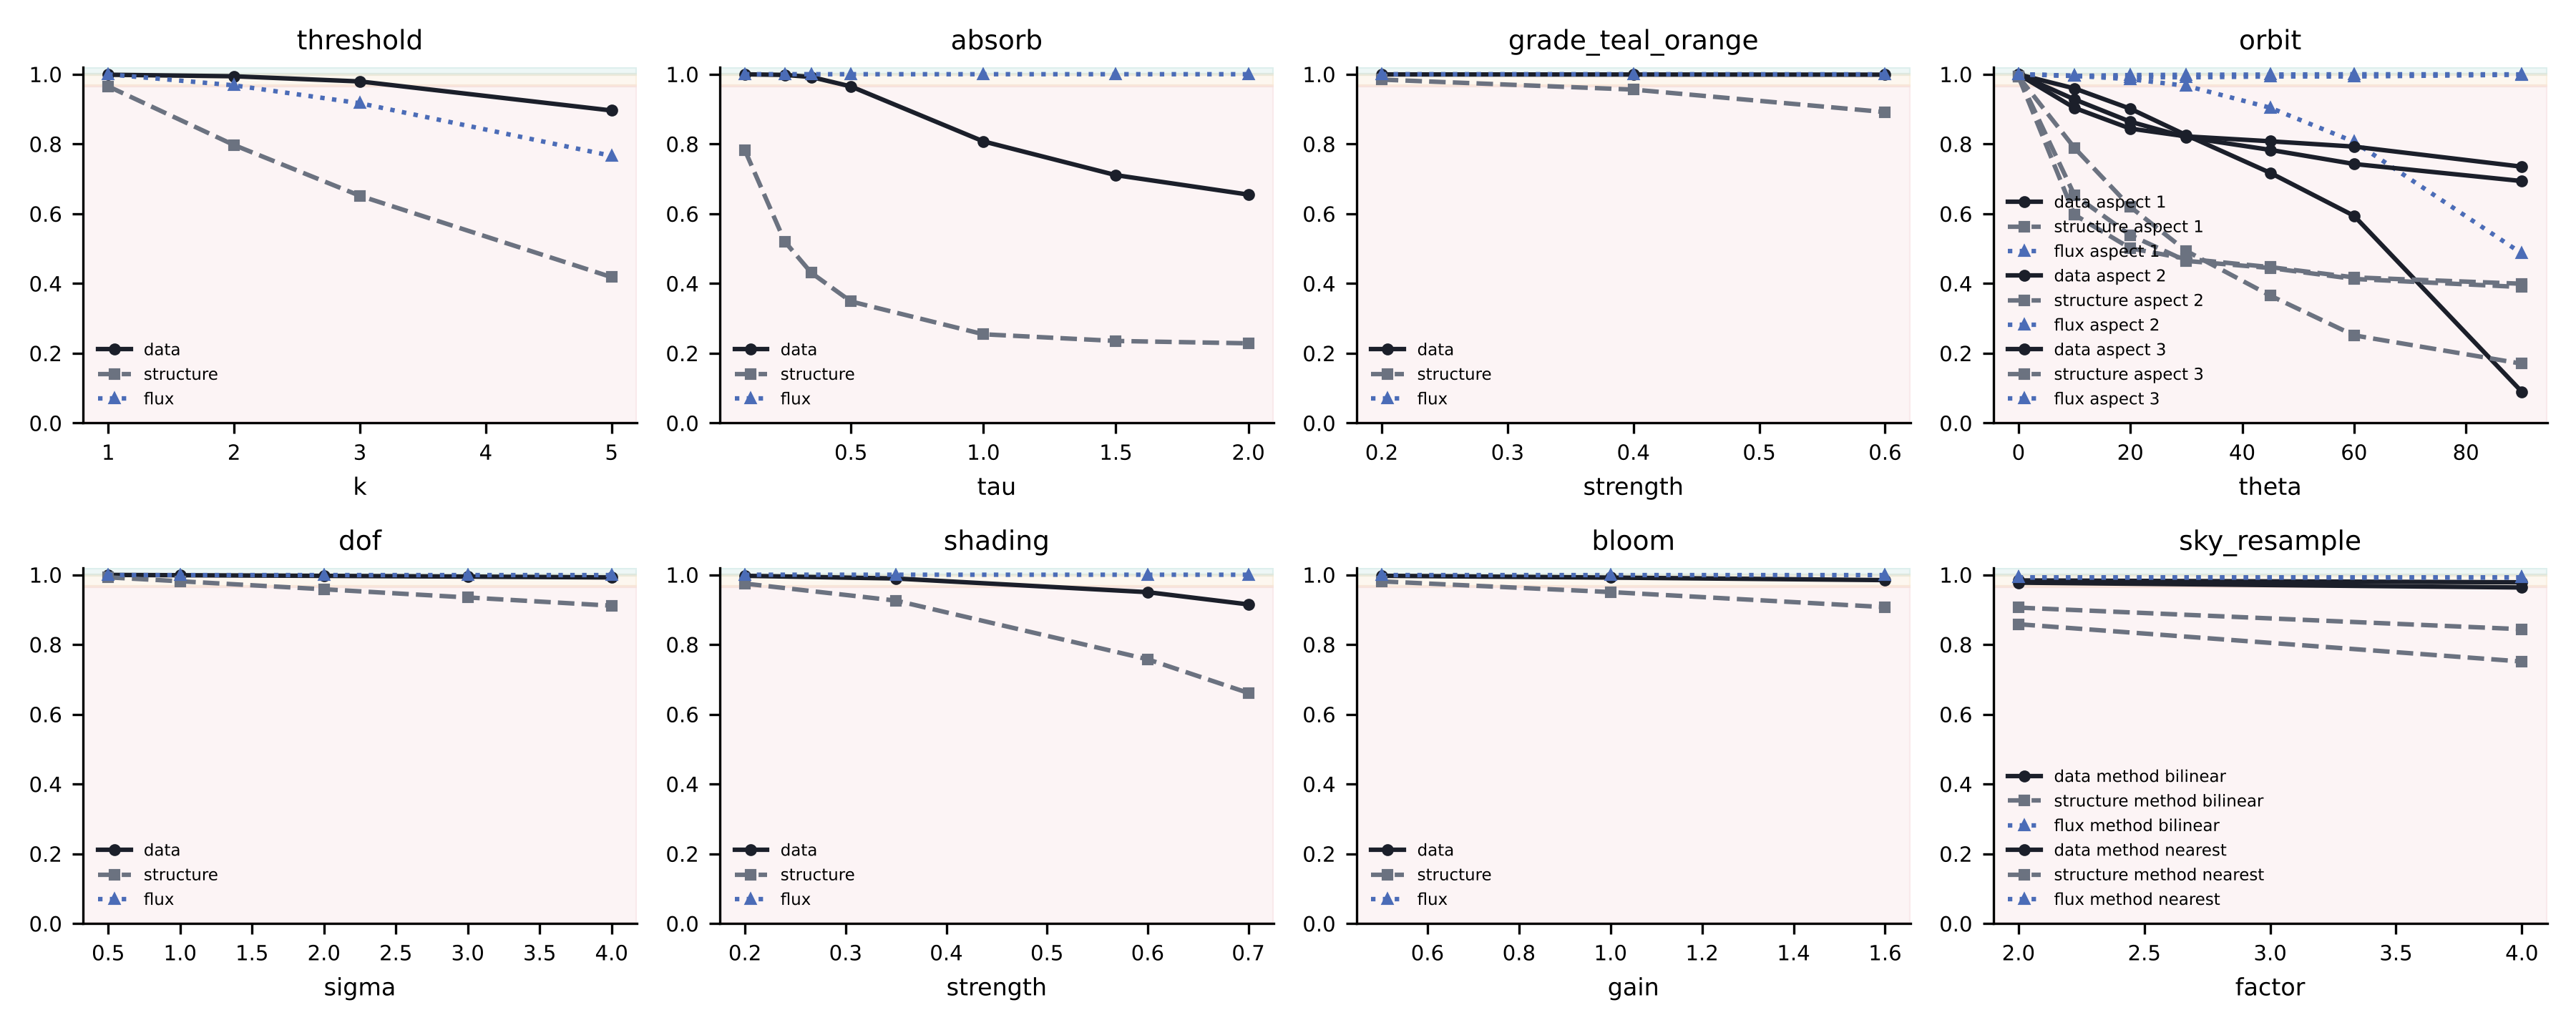
\includegraphics[width=\linewidth]{fig_families_l1448}
  % TODO caption
  \caption{Score vs parameter per family on L1448, bands from the controls.}
  \label{fig:families}
\end{figure}

\begin{figure}[t]
  \centering
  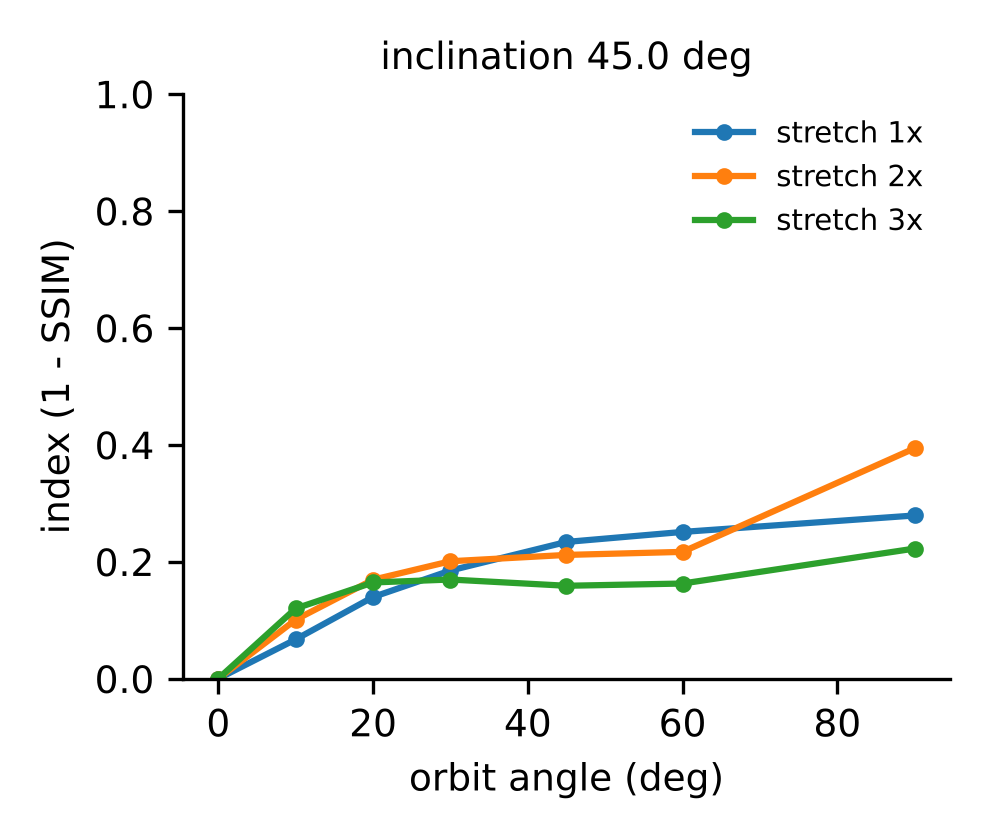
\includegraphics[width=0.6\linewidth]{fig_index}
  % TODO caption
  \caption{Velocity-as-depth index on the synthetic disk vs orbit angle, three stretches.}
  \label{fig:index}
\end{figure}

\section{Discussion and limitations}
% me. machine score != comprehension (bujack 2026, lisnic 2023). jet scores 1.00 for the machine
% and everyone knows it misleads people. only 1 real cube. decoder + band choices. index depends
% on the disk model
\label{sec:discussion}

\section{Future work}
% me. audience study (designed already: 3 fidelity levels x 3 treatments from 1 cube, public vs
% astronomers, beauvis appeal, wang 2025 trust inventory, perceived accuracy, 1 comprehension q,
% pairwise faithfulness, IRB in dec). openvdb carrier into blender. AI pipeline where the pass
% criterion is reproducing the science product (astrovisbench, joseph 2025)
\label{sec:future}

\section{Conclusion}
% arash, 1 paragraph
\label{sec:conclusion}


\bibliographystyle{unsrtnat}
\bibliography{refs}
\end{document}
